%\usetikzlibrary {backgrounds,mindmap}
%\begin{tikzpicture}
%  [root concept/.append style={concept color=blue!80,minimum size=2cm},
%   level 1 concept/.append style={sibling angle=180},
%   level 2 concept/.append style={sibling angle=120},
%   level 3 concept/.append style={sibling angle=90},
%   mindmap]
%  \node [concept] (aeronef) {Aéronef}
%    [clockwise from=0]
%    child[concept color=red] { node[concept] (aerodyne) {Aérodyne}
%    		[clockwise from=90]
%      child[concept color=green] { node[concept] {Voilure fixe} 
%      	[clockwise from=-180]
%      	child[concept color=yellow] { node[concept] {Avion} }
%      	child[concept color=yellow] { node[concept] {Planeur} }
%      	child[concept color=yellow] { node[concept] {Deltaplane} }
%      }
%      child[concept color=green] { node[concept] {Voilure tournante} 
%      	[clockwise from=45]
%      	child[concept color=yellow] { node[concept] {Hélico} }
%      	child[concept color=yellow] { node[concept] {Autogyre} }
%      }
%      child[concept color=green] { node[concept] {Deltaplane} }	
%      }
%    child[concept color=red] { node[concept] (aerostat) {Aérostat}}
%    ;
%\end{tikzpicture}

\section{Classification des aéronefs}
Un \gls{aéronef} \anglais{aircraft} est un appareil capable de s'élever et de se mouvoir au sein de l'atmosphère terrestre. On divise les aéronefs en 2 grandes familles :
\begin{itemize}
	\item les  \gls{aérostat}s \anglais{aerostat/lighter-than-air aircraft}, qui sont des appareils plus légers que l'air,
	\item les  \gls{aérodyne}s \anglais{heavier-than-air aircraft}, qui sont plus lourds que l'air.
\end{itemize}

Dans cette partie, nous étudierons les aéronefs mais également les engins spatiaux. Ceux ci ne peuvent être qualifiés d'aéronefs, car, bien que certains d'entre eux puissent se déplacer dans l'atmosphère, ils peuvent également se mouvoir en dehors de celle-ci.

\subsubsection{Pourquoi classer les aéronefs ?}
Chaque type d'aéronef dispose de propriétés et de contraintes qui lui sont propres. La classification des aéronefs en grand groupes présentant des caractéristiques communes permet de leur associer aisément des notions réglementaires (licence de pilote nécessaire, minima météo, zone de vol autorisées...), techniques (fréquences et mode d'entretien, contraintes de conception) ou administratives (immatriculation, assurance...).

\subsection{Aérostats}
	\subsubsection{Montgolfière}
	La montgolfière \anglais{hot air balloon} est un aérostat gonflé à l'air chaud. \\
	
	Elle est composé d'un ballon (appelé enveloppe) sous lequel est accroché une nacelle dans laquelle prennent place les passagers et le pilote nommé aérostier. Un bruleur généralement alimenté au gaz permet de chauffer l'air contenu dans le ballon. Le pilote chauffe l'air à l'aide du bruleur pour faire monter la montgolfière. \\
	
	La montgolfière ne dispose d'aucun moyen pour se diriger, elle est entièrement soumise aux vents pour ses déplacements. Cependant, le pilote peut exploiter les variation de sens du vent aux différentes altitudes pour orienter son vol dans une certaine mesure.
	
	\begin{figure}[H]
  	\centering
    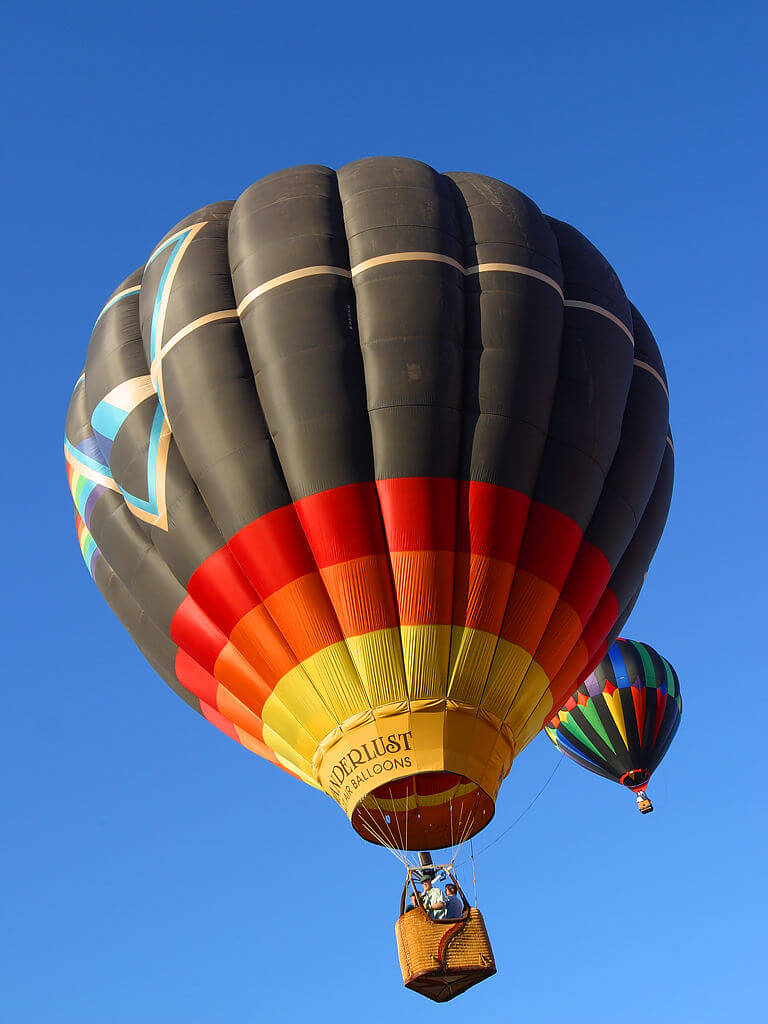
\includegraphics[width=0.4\textwidth]{01-EtudeAeronefs/img/montgolfiere.jpg}
  	\legende{2 ballons dirigeables}{img:montgolfiere}
	\end{figure}	
	
	\histoire{La montgolfière a été le premier aéronef conçu par l'humain. Les frères Montgolfier ont conçu le premier ballon à air chaud et réalisé le premier vol en 1783. La même année, ils font voler des animaux puis Jean-François \textbf{Pilâtre de Rozier} et le Marquis d'Arlandes réalisent le premier vol libre humain. \\ \\ En 1785, Jean-Pierre Blanchard effectue la première traversée de la manche avec un aéronef, 124 ans avant celle effectuée par Louis Blériot en avion.}
	\subsubsection{Ballon à gaz}
	Le ballon à gaz \anglais{gas balloon} est gonflé avec un gaz plus léger que l'air (hydrogène ou hélium).	
	
	\subsubsection{Dirigeable}
	Le dirigeable \anglais{airship} ou ballon dirigeable est un ballon à gaz équipé de systèmes propulsifs lui permettant de se diriger (aussi bien sur le plan horizontal que vertical). \\
	
	Les premiers dirigeables étaient gonflés à l'hydrogène. Ce gaz est dangereux car très inflammable. Les dirigeables modernes sont désormais gonflés à l'hélium. L'hélium est un gaz sûr car ininflammable, mais il est plus cher et plus lourd que l'hydrogène (un ballon à l'hélium nécessitera une enveloppe plus grande qu'un ballon à hydrogène de même capacité).
	
	\info{Il existe également des dirigeables à air chaud.}
	
	\begin{figure}[H]
  	\centering
    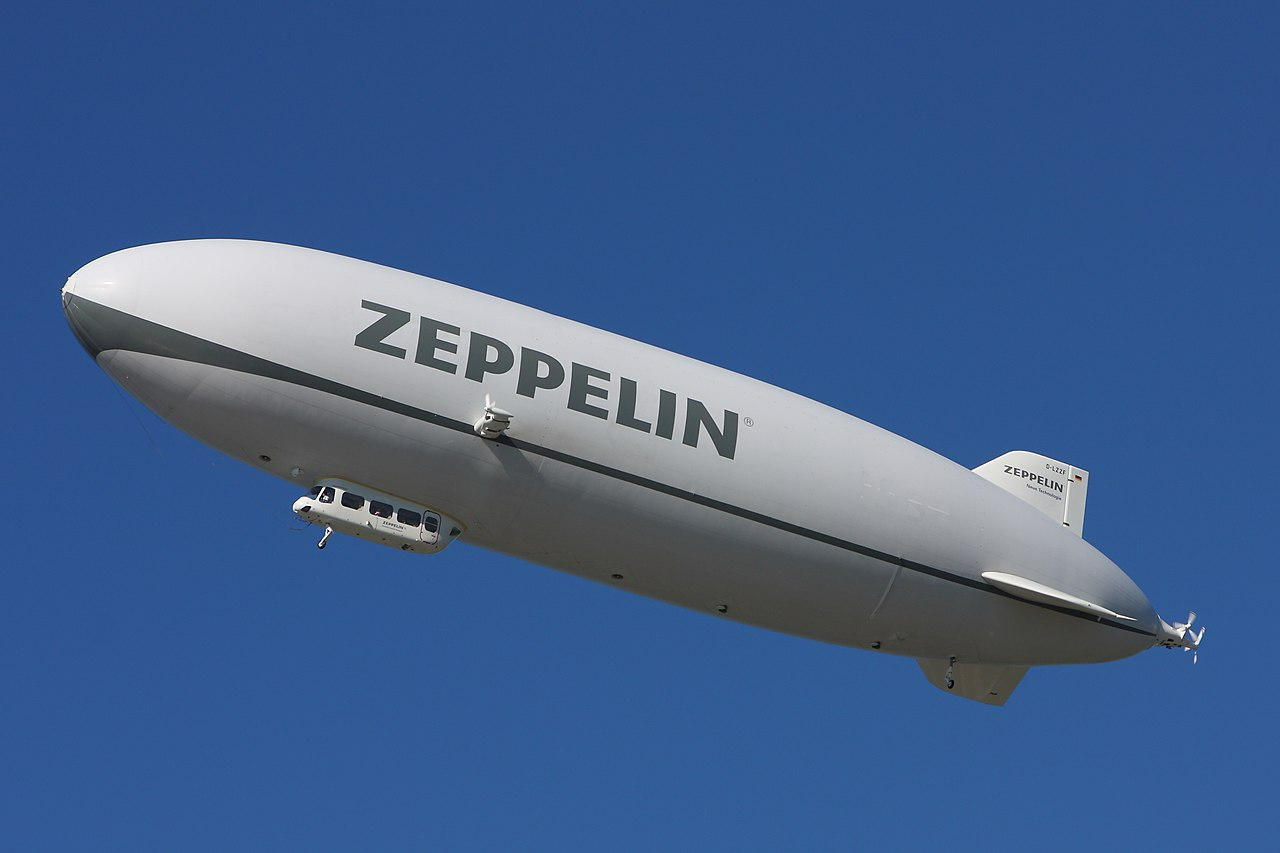
\includegraphics[width=0.4\textwidth]{01-EtudeAeronefs/img/dirigeable.jpg}
  	\legende{Un dirigeable moderne}{img:dirigeable}
	\end{figure}	

\subsection{Aérodynes}
	\subsubsection{Aéronef à voilure fixe}
		Les appareils à voilure fixe \anglais{fixed-wing aircraft}, également appelés aéroplanes sont des aéronefs dont la sustentation est assurée grâce à des phénomènes aérodynamiques sur des surfaces fixes (ailes). Ce type d'aéronef ne peut se maintenir en l'air que si un flux d'air suffisant existe sur ses surfaces portantes.

		\paragraph{Avions}
		La mise en mouvement de l'avion \anglais{airplane} est assuré par son ou ses moteurs. \\
		
		Il existe une très grande diversité de modèles d'avions, variables en taille, vitesse, conception et usages. \\
		
		\histoire{En France, Clément Ader aurait fait voler son Éole dès 1890, mais il n'existe pas de preuve formelle que cet appareil était effectivement quitté le sol. \\ \\  Le premier vol attesté d'un aérodyne à moteur a été réalisé par les frères Wright en 1903 aux États-Unis. C'est cette date qui est officiellement retenue comme celle du premier vol d'un avion.}
	
		\paragraph{Planeurs}
		Le planeur \anglais{glider} est un aérodyne dépourvu de moyens de propulsion. Il est donc dépendant de moyens annexes (remorqueur, treuil) pour sa mise en l'air. \\
		
		Une fois en l'air, le planeur peut exploiter des phénomènes atmosphériques pour gagner de l'altitude. \\
		
		\info{Il existe également des modèles de planeurs équipés de moteurs. Appelés motoplaneurs, ces planeurs peuvent généralement décoller de façon autonome.}
		
		\histoire{Le premier aérodyne à avoir volé est un planeur. Ce vol historique a été réalisé en 1891 par 	\textbf{Otto Lilienthal}.}
		
	\subsubsection{Aéronef à voilure tournante}
	Les appareils à voilure tournante \anglais{rotary-wing aircraft}, également appelés aérogires, sont des aéronefs dont la sustentation est assurée par la rotation d'un ou plusieurs rotors.
	
		\paragraph{Hélicoptères}
		L'hélicoptère \anglais{helicopter} est un aérodyne dont la sustentation est assurée grâce à un rotor entrainé par un moteur.
		
		Les inventeurs qui ont cherché à concevoir les premières hélicoptères au début du \siecle{20} cherchaient à concevoir une machine plus souple que les appareils à voilure fixe en permettant un décollage court voir vertical. 
		
		\histoire{L'idée de la machine à voilure tournante n'est pas récente, puisque l'on dispose de dessins du Léonard de Vinci datés du \siecle{15} représentant des machines à voilures tournantes.}
		
		\paragraph{Autogire}
		L'autogire \anglais{autogyro} est un aérodyne dont la sustentation est assurée grâce à un rotor entrainé par le vent relatif. Les autogires doivent donc dispose d'un mode de propulsion (typiquement une hélice entrainée par un moteur à pistons) qui assure la propulsion de l'appareil sur le plan horizontal.
		
		\histoire{L'autogire à précédé l'hélicoptère. Le premier vol d'un autogire a été effectué en 1923, contre 1936 pour le premier vol réellement contrôlé pour un hélicoptère.}
		
		\paragraph{Convertible}
		Les convertibles \anglais{tiltrotor } sont en quelque sort des hybrides entre des appareils à voilure tournante et des appareils à voilure fixe.
		
		Grâce à des systèmes qui permettent à leurs rotors de basculer d'une position verticale à une position horizontale, ces appareils cherchent à combiner les avantages de l'hélicoptère (vol stationnaire, décollage et atterrissage verticaux) à ceux des appareils à voilure fixe (vitesse de croisière). Cela se fait cependant au prix d'une complexité technique qui rend l'exploitation de ces appareils couteuse et délicate.
		
	\begin{figure}[H]
  	\centering
    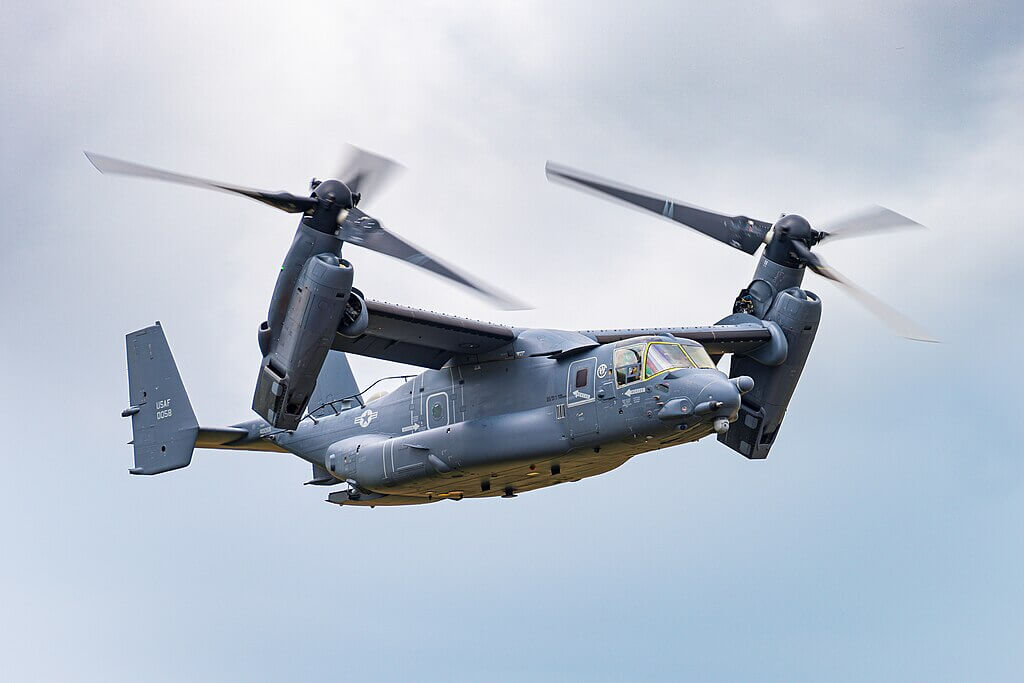
\includegraphics[width=0.4\textwidth]{01-EtudeAeronefs/img/tiltrotor.jpg}
  	\legende{Un convertible : le V22 Osprey}{img:tiltrotor}
	\end{figure}	
		
	\subsubsection{Aéronef à voilure souple}
	Les aéronefs à voilure souple \anglais{flexible wings} regroupent des aéronefs dont la voilure est généralement gonflée par l'air : parapente, paramoteur, parachute sportif moderne... Les deltaplanes rentrent également dans cette catégorie.
	
	\info{Le parachute, dans sa version initiale (coupole), se trouve à a limite de la définition d'un aéronef. En effet, ce type de parachute ne produit pas de portance (uniquement de la traînée) et sa capacité de manœuvre est très limitée.}
	
	\begin{figure}[H]
	\begin{minipage}[c]{0.35\linewidth}
	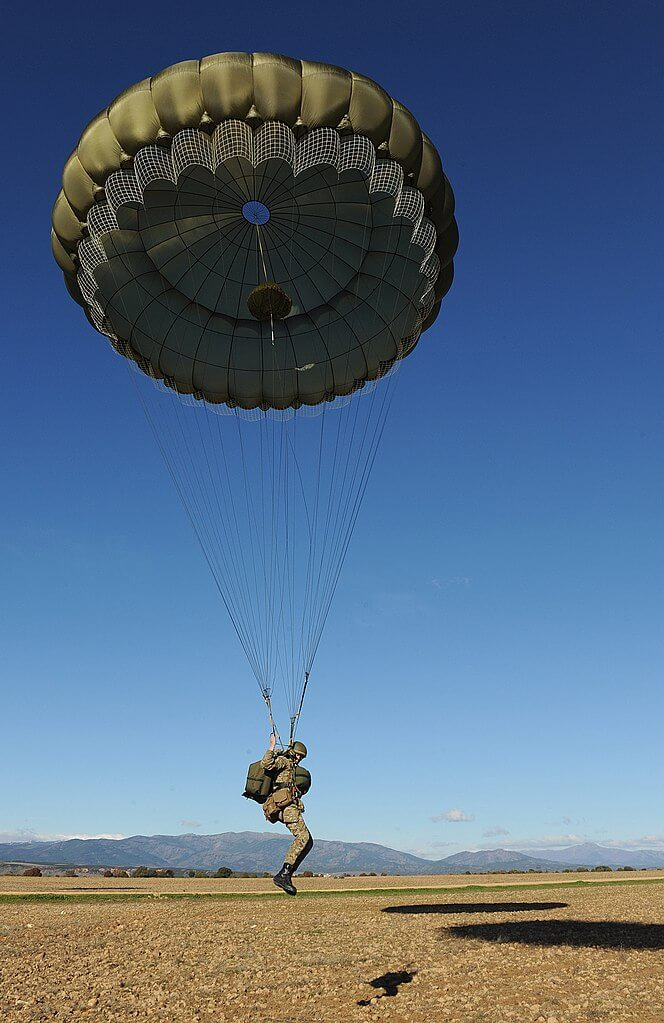
\includegraphics[width=\linewidth]{01-EtudeAeronefs/img/paraMili.jpg}
	\legende{Un parachute coupole}{img:paraMili}
	\end{minipage}
	\hfill
	\begin{minipage}[c]{0.35\linewidth}
	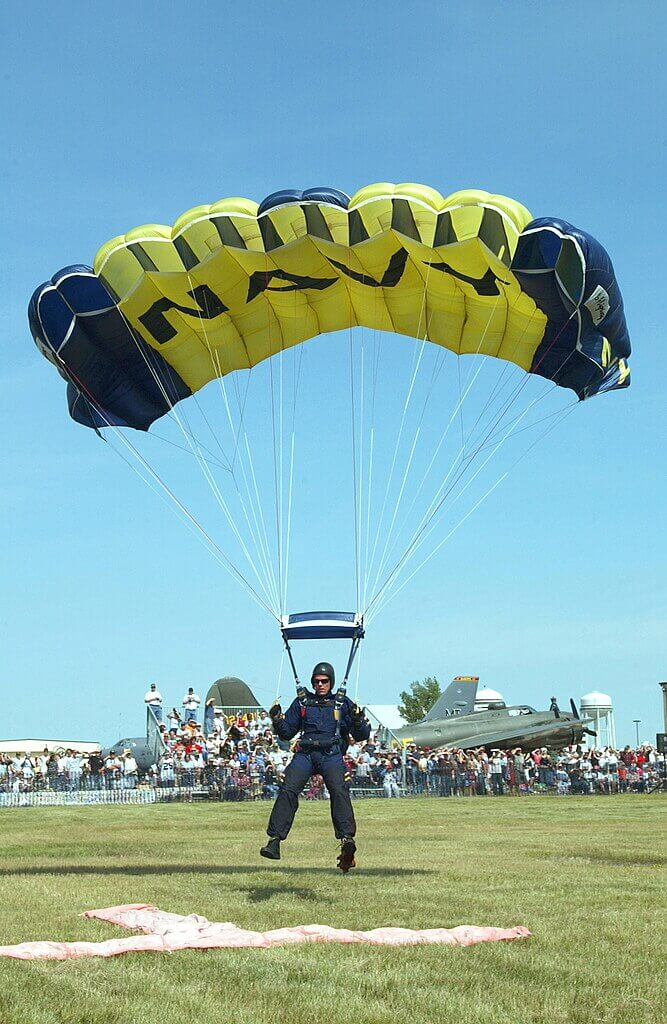
\includegraphics[width=\linewidth]{01-EtudeAeronefs/img/paraSport.jpg}
	\legende{Un parachute sportif moderne}{img:paraSport}
	\end{minipage}
	\end{figure}
	
	\histoire{André-Jacques \textbf{Garnerin}, un ingénieur français, effectue le premier saut réussi en parachute en 1797, en sautant depuis un ballon au dessus de Paris.}
	
\subsection{Engins spatiaux}
	\subsubsection{Lanceurs}
		\paragraph{Fusées}
		\paragraph{Navettes spatiales}
		
	\subsubsection{Engins spatiaux}
		\paragraph{Satellites}
		\paragraph{Sondes}

\subsection{Des grandes familles d'aéronefs}		
\subsubsection{Les ULM}

Les \acrshort{ulm} (\acrlong{ulm}) \anglais{ultralight aircraft} sont un ensemble d'aéronefs motorisés de faible masse. De par cette caractéristique, ils bénéficient de facilités quant à leurs conditions de conception et d'entretien. L'obtention d'une licence de pilote ULM est également simplifiée par rapport aux licences pour des appareils plus lourds (une licence ULM peut s'obtenir après environ 20h de vol). \\

Il existe une grande diversité d'ULM. Il est ainsi possible de piloter des ULM aérostats ou aérondynes, à voilures fixes, tournantes ou souples. En France, ils sont classés en 6 catégories. La licence de pilote d'ULM est commune à toutes les classes, cependant, il faut obtenir une qualification propre à chaque classe, qui permet au pilote de se familiariser avec un instructeur aux particularités propre à chaque type d'aéronef. \\

Chaque classe dispose de ses propres limitations en termes de masse et puissance maximale. Les ULM sont monoplace ou biplace.

	\paragraph{Classe 1 : paramoteur}

	Cette classe est composée d'aérodynes à voilure souple. Elle prend la forme d'un voile type voile de parapente. Le système propulsif, composé d'un moteur et d'une hélice carénée, est soit porté directement dans le dos par le pilote, soit fixé sur un chariot.  
	
	\begin{figure}[H]
  	\centering
    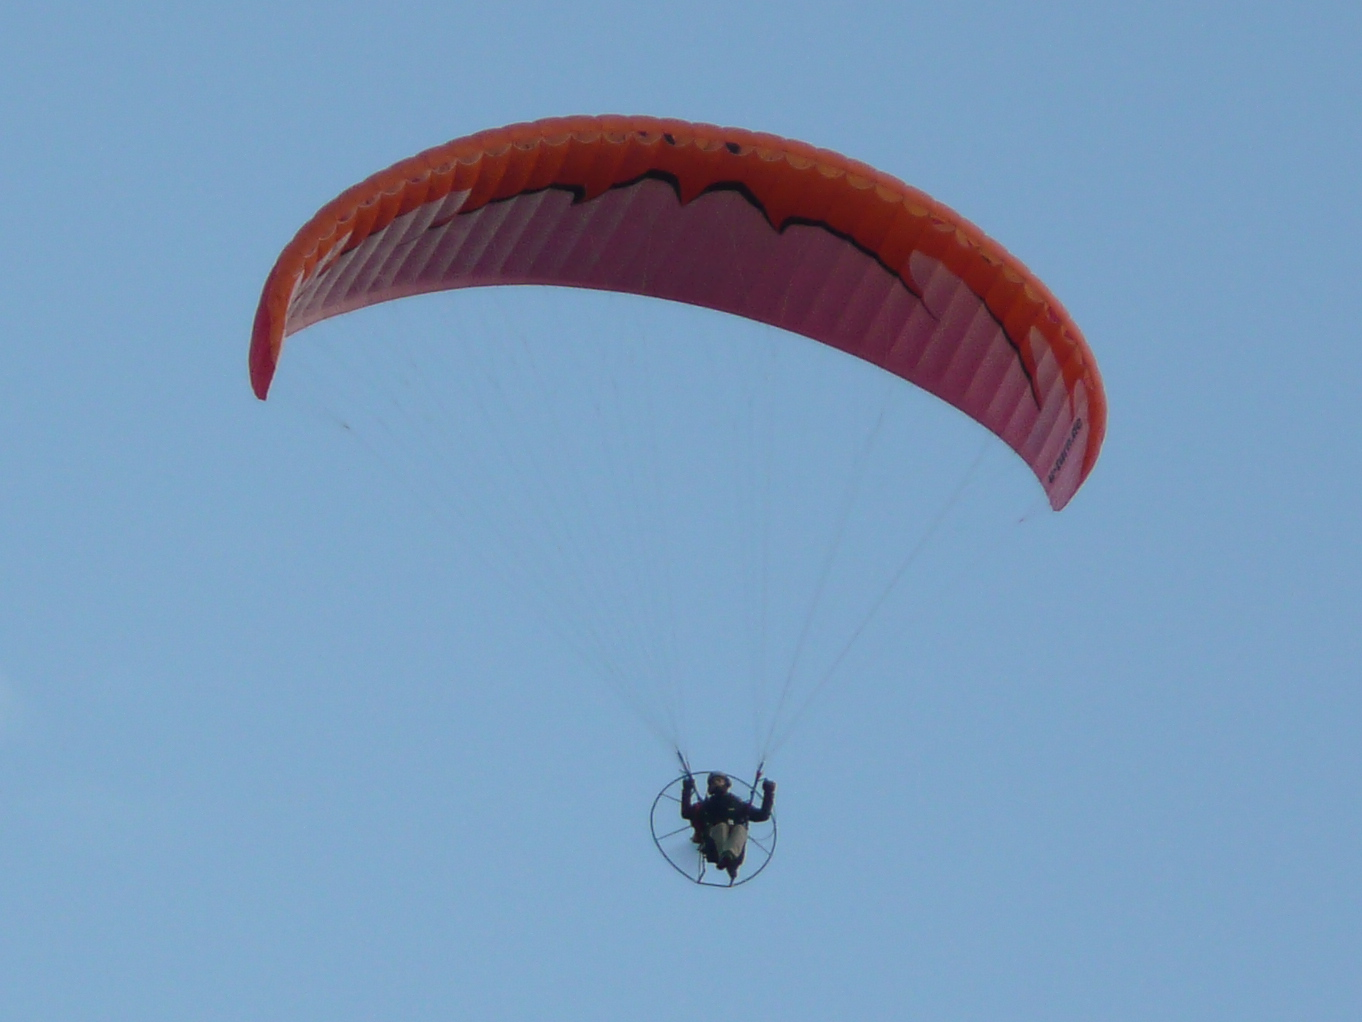
\includegraphics[width=0.4\textwidth]{01-EtudeAeronefs/img/ULM_Classe_1.jpg}
  	\legende{ULM classe 1}{img:ulmClasse1}
	\end{figure}	
	
	\paragraph{Classe 2 : pendulaire}
	Cette classe est composée d'aérodynes constitués de chariots sur lequel est fixé une aile delta. Le nom pendulaire vient du fait que les changements de trajectoires sont obtenus par déplacement du centre de gravité.	
	
	\begin{figure}[H]
  	\centering
    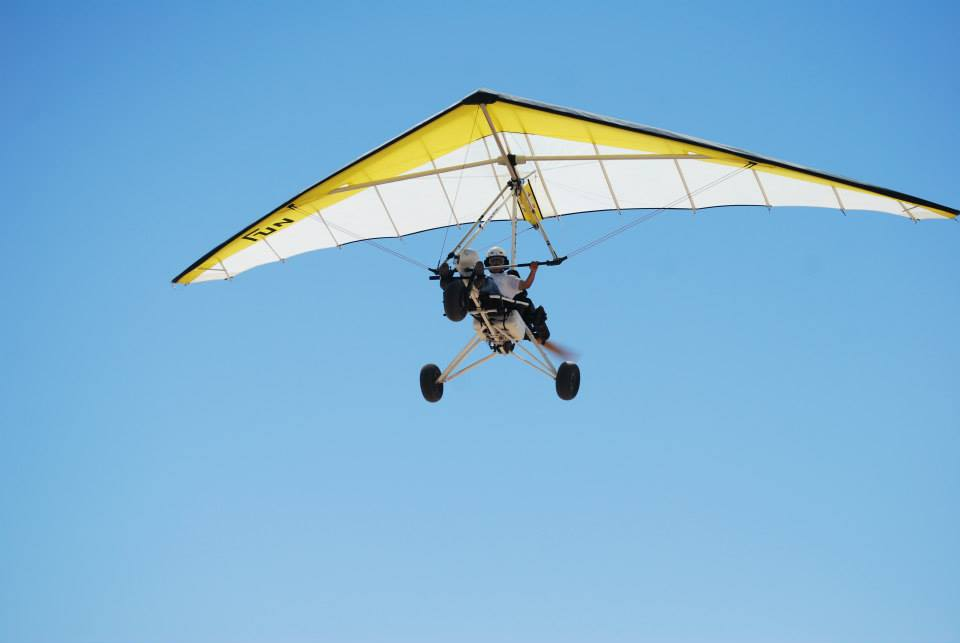
\includegraphics[width=0.4\textwidth]{01-EtudeAeronefs/img/ULM_Classe_2.jpg}
  	\legende{ULM classe 2}{img:ulmClasse2}
	\end{figure}	

	\paragraph{Classe 3 : multiaxes}
	Cette classe est composée d'aérodynes à voilure fixe, qui s'apparentent à des avions traditionnels. Ils est par ailleurs parfois difficile de distinguer un ULM  multiaxe moderne d'un avion biplace.
	
	\info{Aujourd'hui la frontière entre avion et ULM mutliaxes est très réduite. A un telle point que certains fabricants d'avion proposent un même modèle sous la réglementation avion ou ULM en fonction de la masse maximale inscrite sur les documents. C'est le cas de l'ULM présenté en photo ci dessous (commercialisé sous le nom Bristell Classic sous réglementation ULM et Bristel B23 en réglementation avion).}
	
	\begin{figure}[H]
  	\centering
    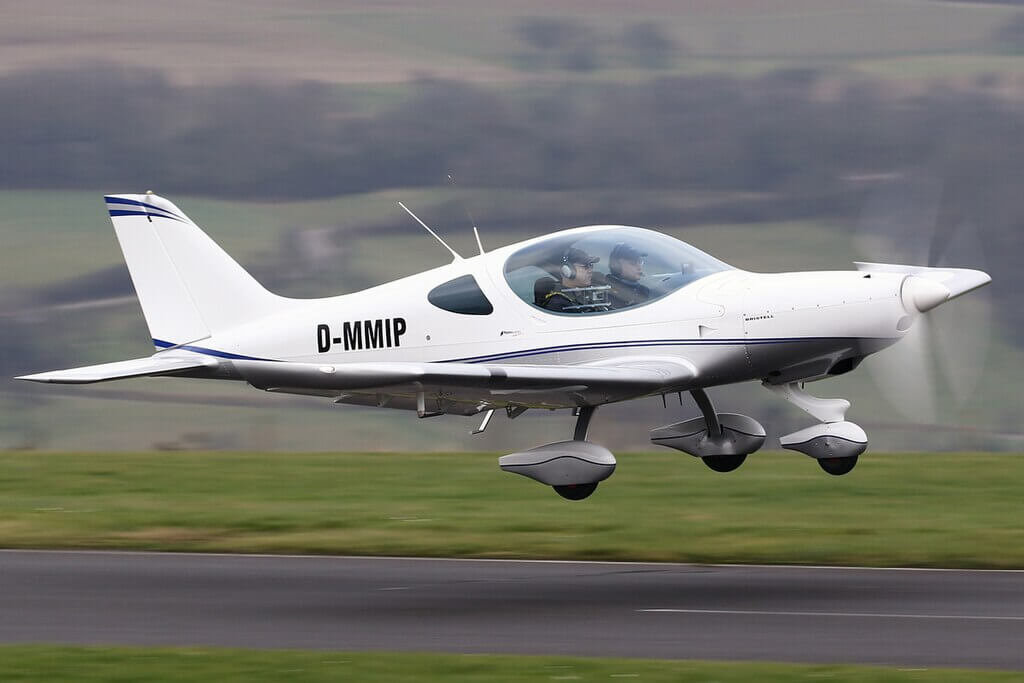
\includegraphics[width=0.4\textwidth]{01-EtudeAeronefs/img/ULM_Classe_3.jpg}
  	\legende{ULM classe 3}{img:ulmClasse3}
	\end{figure}	

	\paragraph{Classe 4 : autogyre}
	Cette classe est composée d'aérodynes à voilure tournante de type autogyres.

	\begin{figure}[H]
  	\centering
    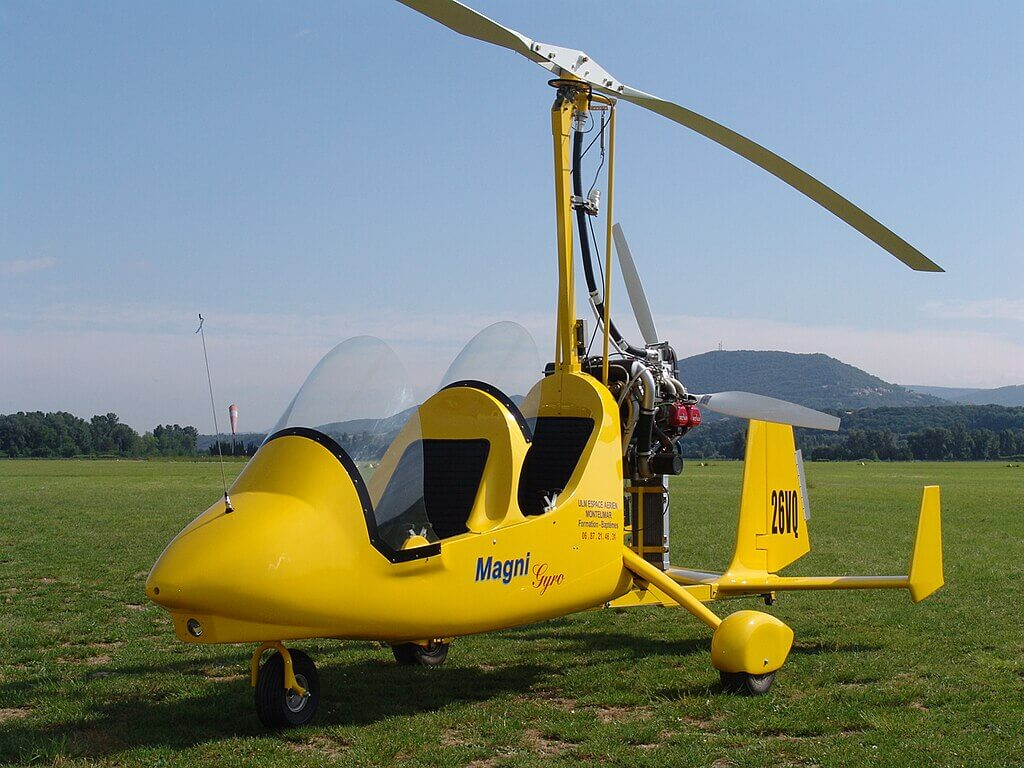
\includegraphics[width=0.4\textwidth]{01-EtudeAeronefs/img/ULM_Classe_4.jpg}
  	\legende{ULM classe 4}{img:ulmClasse4}
	\end{figure}	
	
	\paragraph{Classe 5 : ballon dirigeable}
	Il s'agit d'aérostats dirigeables dont le volume de l'enveloppe est inférieur à 900 m² pour un  ballon à l'hélium et 2000 m² pour les ballons à air chaud.	
	
	\begin{figure}[H]
  	\centering
    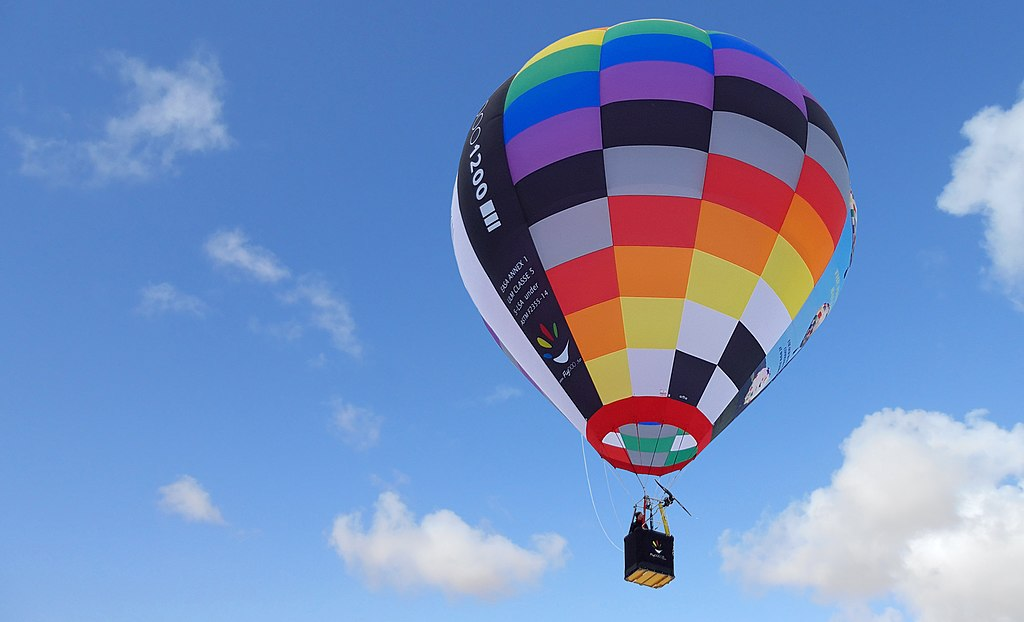
\includegraphics[width=0.4\textwidth]{01-EtudeAeronefs/img/ULM_Classe_5.jpg}
  	\legende{ULM classe 5}{img:ulmClasse5}
	\end{figure}	
		
	\paragraph{Classe 6 : hélicoptère}	
	Dernière née des catégories d'ULM (créer en 2012), cette classe est composée d'aérodynes à voilure tournante de type hélicoptères.
	
	\begin{figure}[H]
  	\centering
    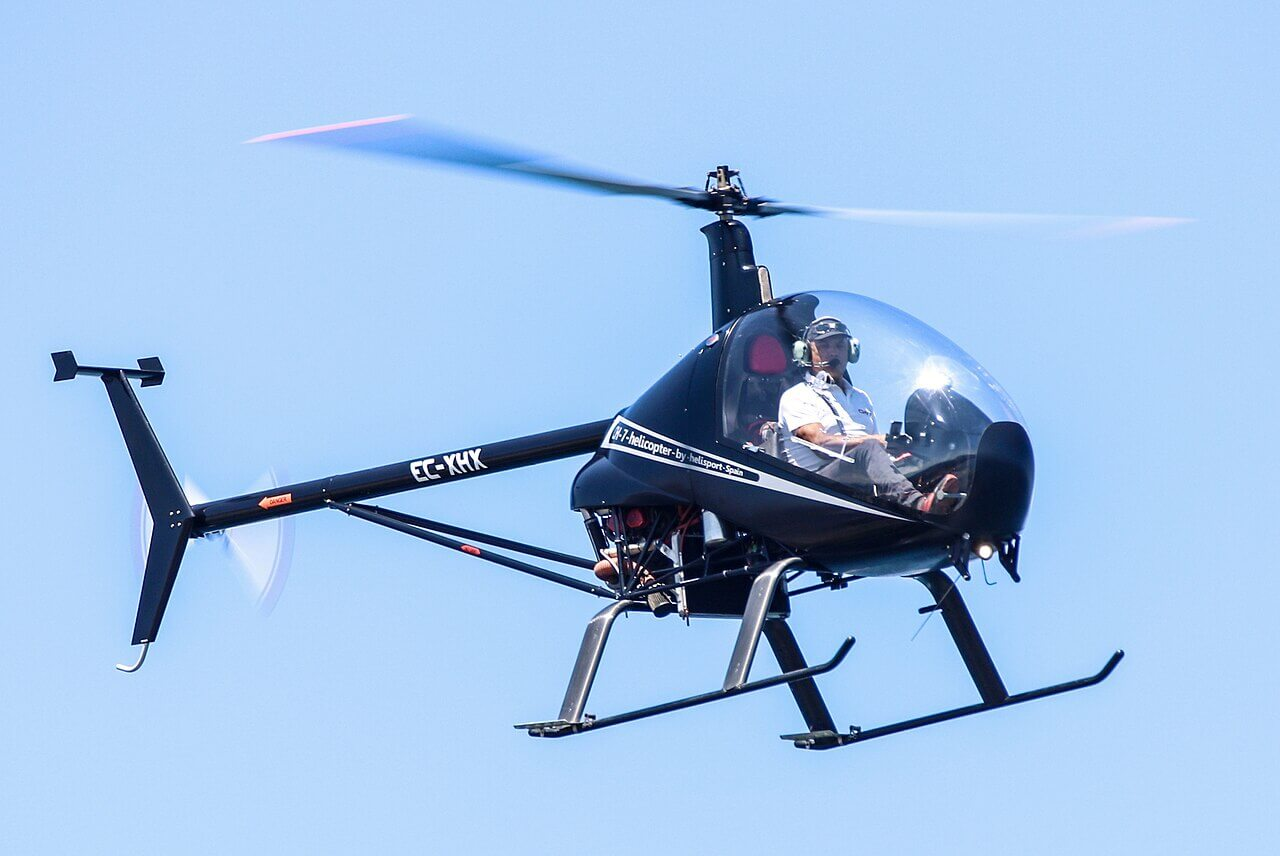
\includegraphics[width=0.4\textwidth]{01-EtudeAeronefs/img/ULM_Classe_6.jpg}
  	\legende{ULM classe 6}{img:ulmClasse6}
	\end{figure}


\subsubsection{Les drones}
Les drones sont des aéronefs pilotés à distance. 

Les drones peuvent être tout type d'aéronef : voilure tournante (typiquement multirotors), voilure fixe, aérostat... Les drones peuvent être libres ou captifs (retenus au sol par un câble).

Il existe également une grande diversité dans les dimensions du drones. Cela va d'appareils mesurant quelques dizaines de centimètre de côté et quelques centaines de grammes à des machines de plusieurs tonnes et de grande envergure. \\

Un système drone est toujours composé de systèmes au sol permettant le contrôle du drone ainsi que du drone lui même. Le drone doit comporter de nombreux systèmes pour assurer son autonomie énergétique, le contrôle de son attitude, le contrôle de sa trajectoire et le suivi de son plan de vol ou encore la liaison dans les 2 sens avec le système de pilotage à distance. 

Enfin, il faut ajouter à ces systèmes les systèmes propres à la mission du drone : capteurs (photo, infrarouge, radio...), systèmes de largage ou d'épandage...
